\documentclass[aspectratio=169,10pt]{beamer}

% ---------- theme & colours ----------
\usetheme{Madrid}
\usecolortheme{whale}
\setbeamertemplate{navigation symbols}{}
\setbeamertemplate{footline}[frame number]
\setbeamerfont{frametitle}{size=\normalsize,series=\bfseries}

% ---------- packages ----------
\usepackage[utf8]{inputenc}
\usepackage[T1]{fontenc}
\usepackage{lmodern}
\usepackage{booktabs}
\usepackage{multirow}
\usepackage{xcolor}
\usepackage{tikz}
\usetikzlibrary{arrows.meta,positioning,fit,shapes.geometric,backgrounds}
\usepackage{colortbl}
\usepackage{array}
\usepackage{amsmath}
\usepackage{graphicx}

% ---------- colour macros ----------
\definecolor{good}{HTML}{c8e6c9}
\definecolor{bad}{HTML}{ffcdd2}
\definecolor{neutral}{HTML}{fff9c4}
\definecolor{mblue}{HTML}{1565C0}
\definecolor{mgray}{HTML}{607D8B}

\newcommand{\good}[1]{\cellcolor{good}#1}
\newcommand{\bad}[1]{\cellcolor{bad}#1}
\newcommand{\neu}[1]{\cellcolor{neutral}#1}

% ---------- title ----------
\title[Prior MoE Attempts for Imbalanced IDS]%
      {Prior MoE Approaches for\\Imbalanced Network Intrusion Detection}
\subtitle{A Review of Attempts Before the \texttt{code\_1/2/3} Series}
\author{Research Summary}
\institute{Network Security \& Class Imbalance Project}
\date{\today}

% =========================================================
\begin{document}
% =========================================================

\begin{frame}
  \titlepage
\end{frame}

% ---------------------------------------------------------
\begin{frame}{Outline}
  \tableofcontents
\end{frame}

% =========================================================
\section{Problem Statement}
% =========================================================

\begin{frame}{Problem: Severely Imbalanced Multi-Class IDS}
  \begin{columns}[T]
    \column{0.52\textwidth}
      \textbf{Datasets}
      \begin{itemize}
        \item CIC-IDS2017 / CIC-IDS2018
        \item UNSW-NB15 / NF-UNSW-NB15
      \end{itemize}
      \vspace{6pt}
      \textbf{Core challenge}
      \begin{itemize}
        \item Imbalance ratio (IR) $> 1{,}000$ for tail attack classes
        \item \textit{Heartbleed}: 9 train samples in CIC-IDS2017
        \item \textit{Infiltration}: 22 train samples
        \item XGBoost baseline already learns benign / head classes well ---
              tail-class recall collapses
      \end{itemize}
      \vspace{6pt}
      \textbf{Goal}
      \begin{itemize}
        \item Beat single XGBoost baseline on \textbf{tail-class F1}
        \item Without sacrificing majority-class precision
      \end{itemize}
    \column{0.44\textwidth}
      \begin{block}{CIC-IDS2017 Tail Classes (val)}
        \footnotesize
        \begin{tabular}{lrr}
          \toprule
          Class & Train $n$ & Baseline Recall \\
          \midrule
          Bot             & 1{,}180 & 0.812 \\
          Heartbleed      &       7 & 0.500 \\
          Infiltration    &      22 & 0.857 \\
          Web-BF          &     905 & 0.847 \\
          Web-SQLi        &      13 & 0.250 \\
          Web-XSS         &     391 & 0.275 \\
          \bottomrule
        \end{tabular}
      \end{block}
  \end{columns}
\end{frame}

% =========================================================
\section{Overview of Attempts}
% =========================================================

\begin{frame}{Timeline of All Prior Attempts}
  \footnotesize
  \renewcommand{\arraystretch}{1.3}
  \begin{tabular}{llll}
    \toprule
    \textbf{Script} & \textbf{Core Idea} & \textbf{Split} & \textbf{Outcome} \\
    \midrule
    \texttt{cic\_6.py}        & Taxonomy-aware MoE (TAILGUARD) & Random & \bad{No gain} \\
    \texttt{cic\_xg\_19.py}   & XGBoost router + SMOTE per expert & Random & \bad{No gain} \\
    \texttt{code\_final.py}   & OOD-filtered competence ensemble  & Random & \bad{No gain} \\
    \texttt{code\_final\_nf.py} & Same on NF-UNSW-NB15            & Random & \neu{Cross-dataset ref.} \\
    \texttt{code\_chrono.py}  & Chronological split (anti-leakage) & Chrono & \bad{Degraded} \\
    \texttt{code\_file.py}    & Per-file split (anti-leakage) & Per-file & \bad{Degraded} \\
    \texttt{code\_mat.py}     & FAR-MoE: CM-derived experts + OOD gating & Chrono & \bad{Val $\approx$1, test no gain} \\
    \bottomrule
  \end{tabular}
  \vspace{8pt}
  \begin{alertblock}{Persistent finding}
    In \emph{every} attempt, the single XGBoost baseline equals or outperforms
    the MoE on the test set.
  \end{alertblock}
\end{frame}

% =========================================================
\section{Attempt 1: TAILGUARD --- \texttt{cic\_6.py}}
% =========================================================

\begin{frame}{\texttt{cic\_6.py} --- TAILGUARD v6.2}
  \begin{columns}[T]
    \column{0.50\textwidth}
      \textbf{Architecture}
      \begin{itemize}
        \item Explicitly maps attack classes to 4 taxonomy groups\\
              (volumetric, slow/low, web, reconnaissance)
        \item One XGBoost expert per group + 5 random specialists
        \item Meta-classifier (Logistic Regression) selects which experts
              to query at inference time
        \item Competence score = $P(\text{expert correct} \mid x)$
      \end{itemize}
      \vspace{6pt}
      \textbf{Training}
      \begin{itemize}
        \item Random stratified 60/20/20 split
        \item Meta-classifier trained on val predictions
      \end{itemize}
    \column{0.46\textwidth}
      \begin{block}{Results (CIC-IDS2017)}
        \footnotesize
        \begin{tabular}{lcc}
          \toprule
          Metric & Baseline & MoE \\
          \midrule
          Accuracy       & 0.9989 & 0.9989 \\
          Macro F1       & 0.8380 & 0.8463 \\
          Weighted F1    & 0.9989 & 0.9989 \\
          \bottomrule
        \end{tabular}
      \end{block}
      \vspace{6pt}
      \begin{alertblock}{Why it failed}
        Router itself misclassifies tail-class samples
        (rare $\Rightarrow$ hard to learn), so those samples are
        routed to the wrong expert and perform \emph{worse} than baseline.
      \end{alertblock}
  \end{columns}
\end{frame}

% =========================================================
\section{Attempt 2: XGBoost Router + SMOTE --- \texttt{cic\_xg\_19.py}}
% =========================================================

\begin{frame}{\texttt{cic\_xg\_19.py} --- XGBoost Router with SMOTE}
  \begin{columns}[T]
    \column{0.50\textwidth}
      \textbf{Key changes from TAILGUARD}
      \begin{itemize}
        \item Router is also an XGBoost (\texttt{multi:softprob}),
              using both original features + per-expert uncertainty
        \item SMOTE applied \emph{per expert} to oversample minority
              classes within each expert's training set
        \item Configurable: \texttt{--assignment\_mode type|random},
              \texttt{--router\_target expert}
        \item Soft routing: each expert weighted by router probability
      \end{itemize}
      \vspace{6pt}
      \textbf{Hypothesis}
      \begin{itemize}
        \item A more powerful router would fix the misrouting problem
        \item SMOTE would alleviate expert-level imbalance
      \end{itemize}
    \column{0.46\textwidth}
      \begin{alertblock}{Root problem exposed}
        XGBoost's boosting \emph{already} implements implicit MoE ---
        it iteratively reweights hard (minority) samples.
        Adding an explicit router on top offers no additional
        specialization signal.
      \end{alertblock}
      \vspace{6pt}
      \begin{block}{Additional failure mode}
        SMOTE within each expert creates synthetic samples that
        may not lie on the true data manifold, and the oversampled
        expert still sees fewer real tail samples than the global model.
      \end{block}
  \end{columns}
\end{frame}

% =========================================================
\section{Attempt 3: OOD Competence Ensemble --- \texttt{code\_final.py}}
% =========================================================

\begin{frame}{\texttt{code\_final.py} --- Drop Routing, Use OOD + Competence}
  \begin{columns}[T]
    \column{0.50\textwidth}
      \textbf{Design shift}: abandon explicit routing
      \begin{itemize}
        \item Each expert always sees all training data
        \item At inference: compute per-expert \emph{OOD score}
              and \emph{competence score}
        \item OOD score: Mahalanobis distance on expert's training
              distribution (LedoitWolf covariance)
        \item Competence: LR trained on val to predict
              ``was this expert correct on this sample?''
        \item Experts with high OOD z-score are excluded;
              remaining experts are weighted by competence
      \end{itemize}
    \column{0.46\textwidth}
      \begin{block}{Results (UNSW-NB15)}
        \footnotesize
        \begin{tabular}{lcc}
          \toprule
          Metric & Baseline & MoE \\
          \midrule
          Accuracy       & 0.8335 & 0.8145 \\
          Macro F1       & 0.5788 & 0.6065 \\
          Weighted F1    & 0.8137 & 0.8215 \\
          \bottomrule
        \end{tabular}
      \end{block}
      \vspace{4pt}
      \begin{alertblock}{Observation}
        Macro F1 improves slightly but \textbf{accuracy drops}.
        Competence model trained on val does not generalise
        to test distribution --- especially under random splits
        where val and test are i.i.d.\ but experts overfit to val.
      \end{alertblock}
  \end{columns}
\end{frame}

% =========================================================
\section{Attempt 4: Temporal Splits --- \texttt{code\_chrono} \& \texttt{code\_file}}
% =========================================================

\begin{frame}{Temporal Splits --- \texttt{code\_chrono.py} \& \texttt{code\_file.py}}
  \begin{columns}[T]
    \column{0.50\textwidth}
      \textbf{Motivation}
      \begin{itemize}
        \item Random stratified splits allow future data to ``leak'' into
              training via shared temporal context (same capture session)
        \item Real-world IDS must generalise to \emph{unseen future attacks}
      \end{itemize}
      \vspace{6pt}
      \textbf{Two strategies}
      \begin{enumerate}
        \item \textbf{Chrono}: within each class, sort by time;
              first 60\% train, next 20\% val, last 20\% test
        \item \textbf{Per-file}: assign whole capture files to
              train/val/test; no sample from the same file in two splits
      \end{enumerate}
    \column{0.46\textwidth}
      \begin{alertblock}{Both strategies degraded performance}
        \begin{itemize}
          \item Tail classes have very few samples; chronological
                ordering leaves test with the ``hardest'' temporal tail
          \item Distribution shift between train and test is large
                under file-wise split
          \item MoE experts specialised on early-time patterns fail
                on later-time attacks even more than the baseline
        \end{itemize}
      \end{alertblock}
      \vspace{4pt}
      \begin{block}{Lesson}
        Preventing leakage is necessary but makes the imbalance problem
        \emph{strictly harder} --- the two problems must be solved jointly.
      \end{block}
  \end{columns}
\end{frame}

% =========================================================
\section{Attempt 5: FAR-MoE --- \texttt{code\_mat.py}}
% =========================================================

\begin{frame}{\texttt{code\_mat.py} --- FAR-MoE Architecture}
  \begin{center}
  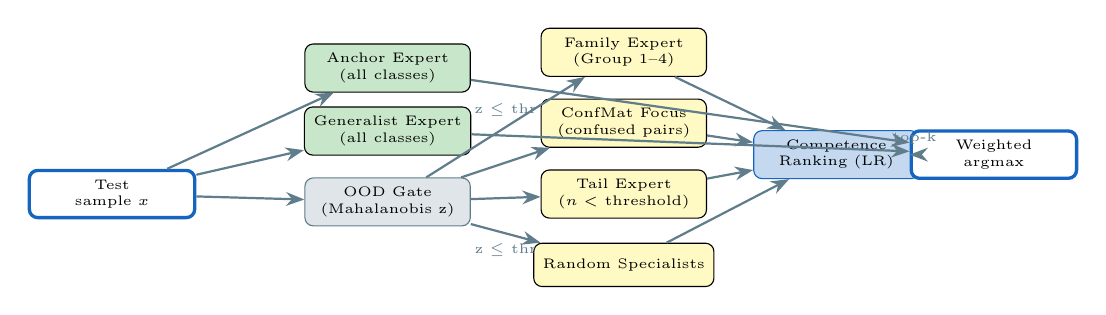
\begin{tikzpicture}[
      box/.style={rectangle,rounded corners=3pt,draw,fill=mblue!15,
                  minimum width=2.1cm,minimum height=0.55cm,
                  font=\tiny,align=center},
      alwaysbox/.style={box,fill=good},
      specialbox/.style={box,fill=neutral},
      arrow/.style={-Stealth,thick,mgray},
      font=\tiny
    ]

    % input
    \node[box,fill=white,draw=mblue,very thick] (inp) at (0,0) {Test\\sample $x$};

    % always-include
    \node[alwaysbox] (anchor)  at ( 3.5, 1.6) {Anchor Expert\\(all classes)};
    \node[alwaysbox] (gen)     at ( 3.5, 0.8) {Generalist Expert\\(all classes)};

    % OOD gate
    \node[box,fill=mgray!20,draw=mgray] (ood) at (3.5,-0.1)
          {OOD Gate\\(Mahalanobis z)};

    % specialists
    \node[specialbox] (fam1) at (6.5, 1.8) {Family Expert\\(Group 1--4)};
    \node[specialbox] (conf) at (6.5, 0.9) {ConfMat Focus\\(confused pairs)};
    \node[specialbox] (tail) at (6.5, 0.0) {Tail Expert\\($n <$ threshold)};
    \node[specialbox] (rand) at (6.5,-0.9) {Random Specialists};

    % competence
    \node[box,fill=mblue!25,draw=mblue] (comp) at (9.2, 0.5)
          {Competence\\Ranking (LR)};

    % output
    \node[box,fill=white,draw=mblue,very thick] (out) at (11.2,0.5)
          {Weighted\\argmax};

    % arrows
    \draw[arrow] (inp)    -- (anchor);
    \draw[arrow] (inp)    -- (gen);
    \draw[arrow] (inp)    -- (ood);
    \draw[arrow] (ood)    -- node[above,font=\tiny]{z $\le$ thr} (fam1);
    \draw[arrow] (ood)    -- (conf);
    \draw[arrow] (ood)    -- (tail);
    \draw[arrow] (ood)    -- node[below,font=\tiny]{z $\le$ thr} (rand);
    \draw[arrow] (fam1)   -- (comp);
    \draw[arrow] (conf)   -- (comp);
    \draw[arrow] (tail)   -- (comp);
    \draw[arrow] (rand)   -- (comp);
    \draw[arrow] (anchor) -- (out);
    \draw[arrow] (gen)    -- (out);
    \draw[arrow] (comp)   -- node[above,font=\tiny]{top-k} (out);

  \end{tikzpicture}
  \end{center}
  \vspace{-4pt}
  \scriptsize
  \textbf{Feature views} per expert: \texttt{volume} (byte/packet counts),
  \texttt{timing} (IAT, duration), \texttt{packet} (flag/size),
  \texttt{tcp}, \texttt{all}.
  \quad \textbf{ConfMat Focus}: confusion pairs derived from a baseline probe
  on the \emph{validation} split.
\end{frame}

\begin{frame}{\texttt{code\_mat.py} --- FAR-MoE Results \& Failure Mode}
  \begin{columns}[T]
    \column{0.50\textwidth}
      \textbf{Selected per-class results (CIC-IDS2017 test)}
      \footnotesize
      \renewcommand{\arraystretch}{1.2}
      \begin{tabular}{lcc}
        \toprule
        Class & Recall(B) & Recall(MoE) \\
        \midrule
        Web-XSS      & 0.231 & \good{0.838} \\
        Bot          & 0.756 & \good{0.804} \\
        Web-BF       & 0.850 & \bad{0.502} \\
        Web-SQLi     & 0.000 & 0.000 \\
        Infiltration & 0.571 & 0.571 \\
        \midrule
        Macro F1     & 0.838 & \neu{$\approx$same} \\
        \bottomrule
      \end{tabular}
      \normalsize
      \vspace{6pt}
      Some tail classes improve, others regress --- net effect is neutral.
    \column{0.46\textwidth}
      \begin{alertblock}{Critical failure: CM leakage}
        \begin{itemize}
          \item The ConfMat Focus expert is designed using the \emph{confusion
                matrix on the validation split of the same dataset}
          \item Confusion patterns on val $\neq$ confusion patterns on test,
                especially under chronological splits
          \item Val accuracy looks near-perfect
                (probe sees similar distribution as its own training set)
          \item At test time, the "focus expert" targets the wrong class pairs
        \end{itemize}
      \end{alertblock}
  \end{columns}
\end{frame}

% =========================================================
\section{Failure Analysis}
% =========================================================

\begin{frame}{Consolidated Failure Analysis}
  \renewcommand{\arraystretch}{1.35}
  \footnotesize
  \begin{tabular}{lp{5.8cm}p{4.0cm}}
    \toprule
    \textbf{\#} & \textbf{Failure Mode} & \textbf{Observed in} \\
    \midrule
    1 &
    \textbf{Routing error compounds imbalance.}
    Tail classes are rare $\Rightarrow$ router cannot learn them $\Rightarrow$
    tail samples routed to wrong expert $\Rightarrow$ worse than baseline. &
    \texttt{cic\_6}, \texttt{cic\_xg\_19} \\[4pt]
    2 &
    \textbf{Expert-level imbalance unresolved.}
    Partitioning classes across experts does not change the within-expert IR;
    each specialist still sees too few tail samples to specialise. &
    All MoE variants \\[4pt]
    3 &
    \textbf{CM leakage / val overfitting.}
    Confusion-matrix-derived expert design exploits val distribution;
    patterns do not transfer to test (especially chrono/file splits). &
    \texttt{code\_mat} \\[4pt]
    4 &
    \textbf{XGBoost implicit MoE.}
    Gradient boosting already reweights hard examples iteratively.
    Explicit routing adds overhead but no new specialisation signal. &
    All MoE variants \\
    \bottomrule
  \end{tabular}
\end{frame}

% =========================================================
\section{Summary \& Open Questions}
% =========================================================

\begin{frame}{Summary: What We Know}
  \begin{columns}[T]
    \column{0.48\textwidth}
      \textbf{Negative results (confirmed)}
      \begin{itemize}
        \item Taxonomy-based routing $\Rightarrow$ no gain
        \item XGBoost router + SMOTE $\Rightarrow$ no gain
        \item OOD + competence weighting $\Rightarrow$ no gain
        \item Confusion-matrix expert design $\Rightarrow$ val leakage
        \item Temporal splits make imbalance harder, not easier
      \end{itemize}
    \column{0.48\textwidth}
      \textbf{Open research questions}
      \begin{enumerate}
        \item \textbf{Unbiased expert design:} how to partition classes into
              experts such that each expert genuinely sees different
              feature-space structure, not just different class labels?
        \item \textbf{Routing under imbalance:} can a router be trained
              without seeing tail classes, yet still route them correctly?
        \item \textbf{Leakage-free temporal evaluation:} how to design an
              ensemble that improves \emph{and} degrades gracefully under
              distribution shift?
        \item \textbf{Beyond XGBoost:} does the implicit-MoE argument hold
              for other base learners (LightGBM, CatBoost, neural nets)?
      \end{enumerate}
  \end{columns}
  \vspace{10pt}
  \begin{block}{Next: \texttt{code\_1/2/3} series}
    Address the unbiased expert design problem directly
    by \ldots\ (see subsequent slides)
  \end{block}
\end{frame}

\begin{frame}{Appendix: Experiment Settings}
  \footnotesize
  \renewcommand{\arraystretch}{1.25}
  \begin{tabular}{ll}
    \toprule
    \textbf{Setting} & \textbf{Value} \\
    \midrule
    Base learner       & XGBoost (\texttt{multi:softprob}) \\
    Split (random)     & Stratified 60 / 20 / 20 \\
    Split (chrono)     & Episode-based attack, chronological normal 60/20/20 \\
    Split (per-file)   & Whole capture files assigned to train/val/test \\
    SMOTE threshold    & 1{,}000 samples per class \\
    OOD model          & LedoitWolf covariance $\Rightarrow$ Mahalanobis distance \\
    Competence model   & Logistic Regression on val \\
    Random seed        & 42 \\
    Datasets           & CIC-IDS2017, UNSW-NB15, NF-UNSW-NB15 \\
    \bottomrule
  \end{tabular}
\end{frame}

\end{document}
